% !TEX TS-program = pdflatex
% !TEX encoding = UTF-8 Unicode

% This is a simple template for a LaTeX document using the "article" class.
% See "book", "report", "letter" for other types of document.

\documentclass[11pt]{article} % use larger type; default would be 10pt

\usepackage[utf8]{inputenc} % set input encoding (not needed with XeLaTeX)

%%% Examples of Article customizations
% These packages are optional, depending whether you want the features they provide.
% See the LaTeX Companion or other references for full information.

%%% PAGE DIMENSIONS
\usepackage{geometry} % to change the page dimensions
\geometry{letterpaper} % or letterpaper (US) or a5paper or....
% \geometry{margin=2in} % for example, change the margins to 2 inches all round
% \geometry{landscape} % set up the page for landscape
%   read geometry.pdf for detailed page layout information

\usepackage{graphicx} % support the \includegraphics command and options
\graphicspath{{fig/}}

%%% PACKAGES
\usepackage{booktabs} % for much better looking tables
\usepackage{array} % for better arrays (eg matrices) in maths
\usepackage{paralist} % very flexible & customisable lists (eg. enumerate/itemize, etc.)
\usepackage{verbatim} % adds environment for commenting out blocks of text & for better verbatim
\usepackage{subfig} % make it possible to include more than one captioned figure/table in a single float
\usepackage{gensymb} % general symbols
\usepackage{amsmath} % math symbols
\usepackage{amsfonts} % for symbols
\usepackage{amssymb} % for symbols
\usepackage{placeins}% to prevent floating between sections
\usepackage{subfig} % for subfloats
\usepackage{epstopdf} % for including EPS files
\usepackage{lpic}



% These packages are all incorporated in the memoir class to one degree or another...

%%% HEADERS & FOOTERS
\usepackage{fancyhdr} % This should be set AFTER setting up the page geometry
\pagestyle{fancy} % options: empty , plain , fancy
\renewcommand{\headrulewidth}{0pt} % customise the layout...
\lhead{}\chead{}\rhead{}
\lfoot{}\cfoot{\thepage}\rfoot{}

%%% SECTION TITLE APPEARANCE
\usepackage{sectsty}
\allsectionsfont{\sffamily\mdseries\upshape} % (See the fntguide.pdf for font help)
\setcounter{secnumdepth}{-1}
% (This matches ConTeXt defaults)

%%% ToC (table of contents) APPEARANCE
\usepackage[nottoc,notlof,notlot]{tocbibind} % Put the bibliography in the ToC
\usepackage[titles,subfigure]{tocloft} % Alter the style of the Table of Contents
\renewcommand{\cftsecfont}{\rmfamily\mdseries\upshape}
\renewcommand{\cftsecpagefont}{\rmfamily\mdseries\upshape} % No bold!

%%% Custom Commands and Parameters
\providecommand{\e}[1]{\ensuremath{\times 10^{#1}}}
\newcolumntype{C}[1]{>{\centering\let\newline\\\arraybackslash\hspace{0pt}}m{#1}}

%%% END Article customizations

%%% The "real" document content comes below...

\title{Analog Electronics Final Project Report}
\author{Ankur Dhar and James Ryan Schloss}
\date{\today} % Activate to display a given date or no date (if empty),
         % otherwise the current date is printed 

\begin{document}
\maketitle
\section{Overview}

\section{Mechanical Design}
\begin{itemize}
\item Motors x4
\item ESC x4
\item Battery
\item Central control board (4x5 inches)
\item TTL board x4
\end{itemize}
\begin{figure}[h]
\centering
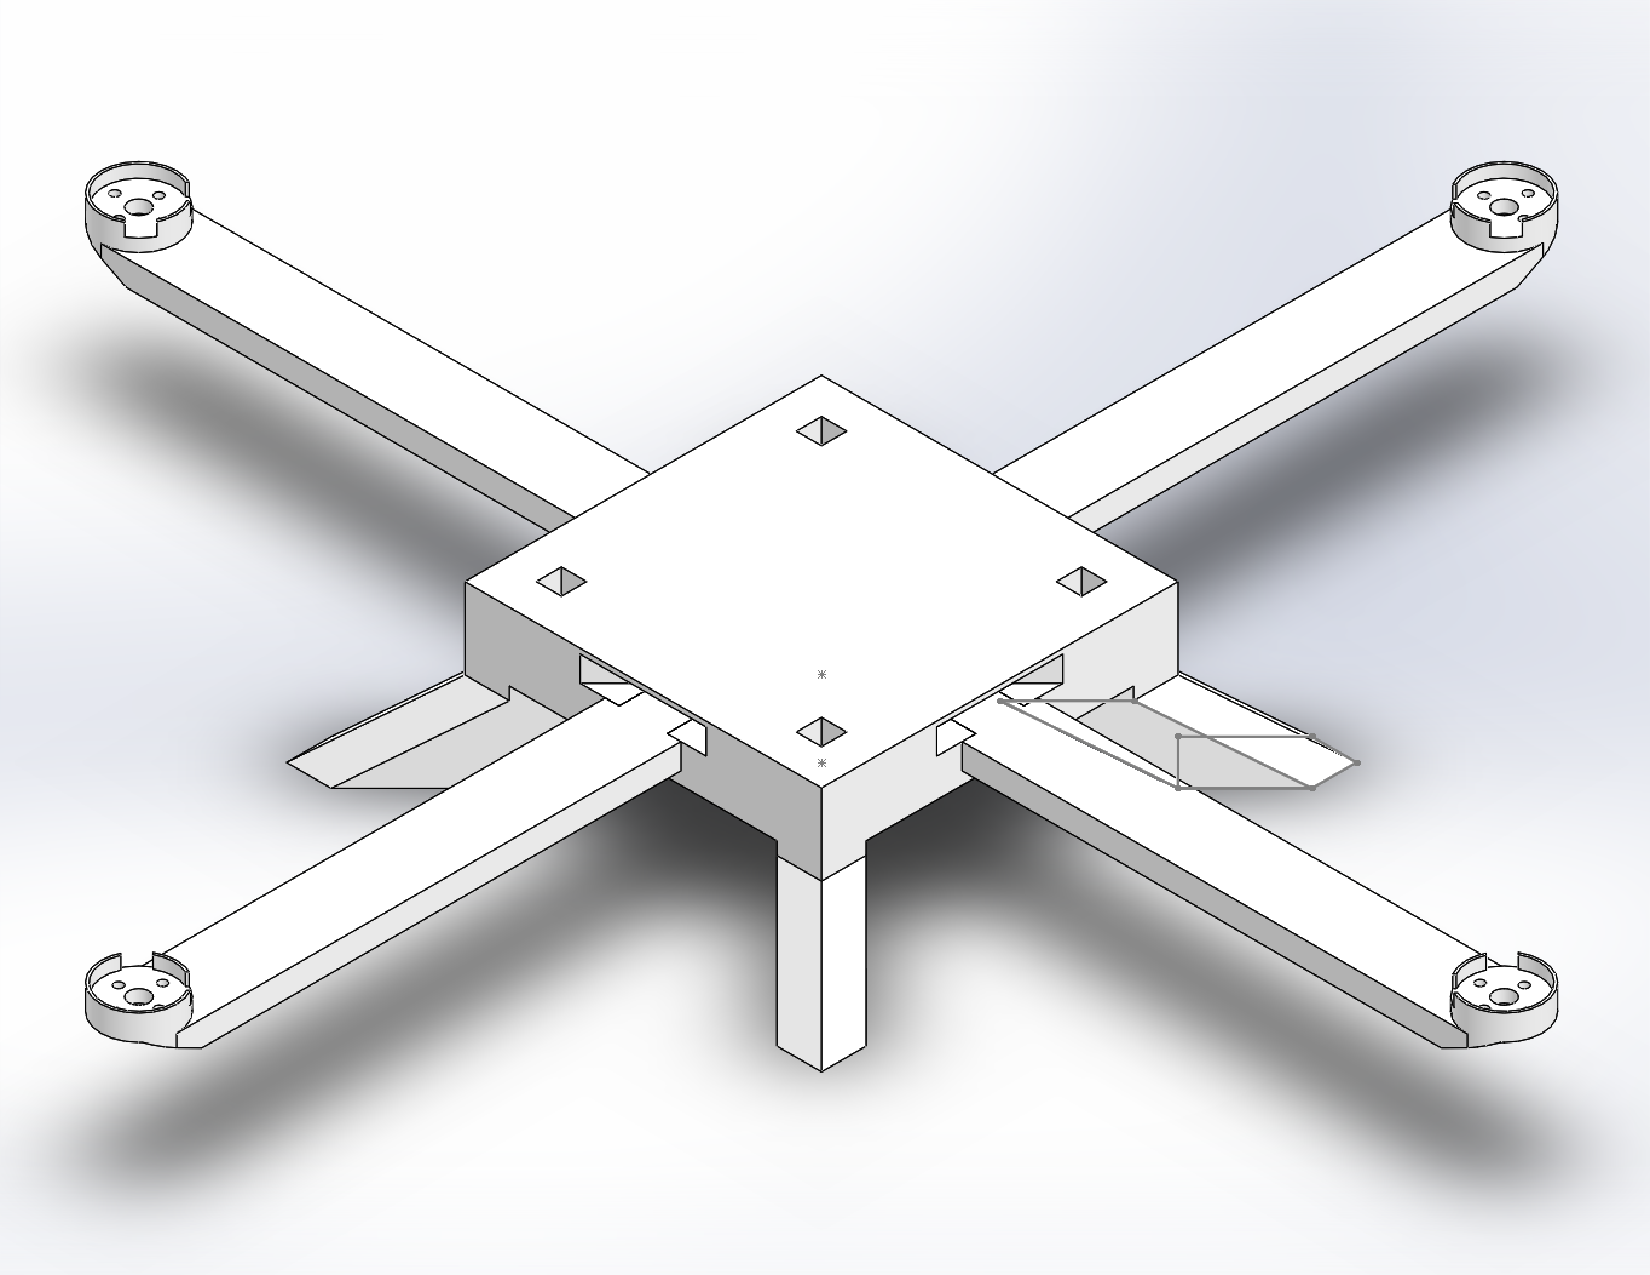
\includegraphics[width=\textwidth]{Quadcopter2D}
\caption{3D render of quadcopter chassis, with room for motors, battery, and requisite electronics.}
\end{figure}
\section{Control Circuit}
Accelerometer outputs voltage proportional to acceleration in X,Y,Z
Thus the equilibrium position is (0,0,-g)
To determine this equilibrium, we integrate the signal twice to determine to displacement, and select for the height we wish to hover at with a comparator. We also select for zero velocity in x and y with this method.
\section{Motor Control}
These output voltages are scaled to range between 2 and 4V, thus varying the throttle of the motor.
\section{Feedback}
 The feedback mechanism in this case is not electrical, but connected through the orientation of the copter, and how it'll affect the output of the accelerometer.
\\
Motors driven by 3 phase signal with the third phase shift set by back emf\\
ESC manages this driving signal, but requires a TTL signal to control throttle\\
Range from 4V to 2V for Duty cycle 25\% to 65\%\\
Triangle wave needs 2.5V offset, with 4V p-p
\section{Problems and Issues}

\section{Conclusion}

\appendix
\section{Characterizing Motors}
\end{document}
